\chapter{Engineering Economics}\label{ch-eng-econ}

Engineers have to consider the cost of the items designed, thus we must know some economics.  This is an introduction to engineering economics.  Those regularly dealing with costing are encouraged to study other references for a deeper coverage.  This should get you started though.

\section{Financial Preliminaries}
Some standard variables I will use are:

\begin{description}
\item[$P$] Present sum of money, sometimes called principle though this does not always make sense.
\item[$F$] Future sum of money, at $n$ periods in the future.
\item[$A$] Annuity, or regular payment of the same amount.
\item[$G$] Geometric payment series.
\item[$i$] Interest rate per compounding period, usually a year.
\item[$n$] Number of interest periods.
\item[$r$] Nominal interest rate per year, does not consider effect of subperiod compounding.
\item[$m$] Number of compounding subperiods.
\end{description}


\subsection{Simple Interest}
We want to study finance, and to do so we must look at interest.  The most basic kind of interest is simple interest.  While not used in the US, simple interest is used in some countries in Africa.  Let's get a few terms down first.
\begin{description}
\item[Principle (P)] the amount borrowed or initial balance.
\item[Future worth (F)] worth of the investment at that interest rate.
\item[Interest rate (i)] the percent of the principle charged for the loan.
\end{description}
The interest charged each year is the same in simple interest, and can be found by multiplying the interest rate times the amount owed, $Pi$.  Simple interest is an example of arithmetic growth.  The series that shows how much must be paid for  a simple interest loan of $P$ at rate $i$ for $n$ years is
\begin{eqnarray}
F &=& P + Pi + Pi + \cdots + Pi \nonumber\\
  &=& P + nPi \nonumber\\
  &=& P(1+ni)
\end{eqnarray}

\subsection{Compound Interest}
In the US we do not use simple interest, but rather compound interest.  Before we get into the formal ideas, let's see why it is called compound interest.

Say you put $P$ dollars in a savings account at an interest rate of $i$.  We will assume the interest is calculated and added to your account only once a year.  The interest earned at the end of the year is $Pi$, just as in simple interest.  After $1$ year you have $P(1+i)$ dollars.  If you leave the money in the account then the next year you will have a new initial amount of $P(1+i)$, so the interest paid will be $(P(1+i))i$.  The total money you have will be $P(1+i)(1+i)=P(1+i)^2$.  As this continues, the money you have at the end of $n$ years is
\begin{eqnarray}
F   &=& P(1+i)^n.
\end{eqnarray}
The interest builds upon itself to help you, or compound your gain.

We do not have to compound (or add) the interest just once a year, you can compound a number of times a year.  Say we compounded interest $m$ times per year, at the end of a year we would have $P(1+i)^m$ dollars, right?. Interestingly (pardon the pun) no bank uses the same $i$ in yearly interest compounding as in more frequent compounding.  The interest used when interest is compounded more than once a year is $r=\frac{i}{m}$.  If a bank lists that an account pays a nominal (APR) of $i=rm$ that is compounded $m$ times per year, the rate used in the compounding equation is $r$.  The formula reads $P(1+ \frac{i}{m})^m=P(1+r)^m$.  If we leave our money in for two years we would have $P(1+ \frac{i}{m})^{2m}=P(1+r)^{2m}$.  Sometimes instead of listing the nominal interest (APR), a bank will list the effective rate (APY).  This comes from noticing that $(1+r)^m>1$, so we can write it as $(1+r)^m=1+r_e$.  We then solve for $r_e$ to find that $r_e=(1+r)^m-1$.  You would have this actual interest rate if the account were compounded annually.  After $n$ years, the balance will have grown to
\begin{eqnarray}
F &=& P(1+ \frac{i}{m})^{nm} \\
  &=&P(1+r)^{nm} \\
  &=&P(1+r_e)^{n}.
\end{eqnarray}
This series is a geometric series.  This is a commonly calculated equation, so we will do a little bit of work to get it into an even more useful form.
\begin{eqnarray}
F &=& P(1+r)^{k}\nonumber\\
\frac{F}{P} &=& (1+r)^{k}\\
            &=& \left(F/P,\;r,\;k\right) \label{eq-single-payment-compounded}
\end{eqnarray}
The final equation (eq.~\ref{eq-single-payment-compounded}) is called the \textbf{single payment compound amount factor}, and is tabulated in many places for different interest rates.  This allows for easy calculation.  It is also easy to code the formula for programs.

\subsubsection{Easy Estimation}

One challenge with compounded interest is estimating what something is worth in 20 years at some interest rate.  There is an easy way to estimate this value.
\begin{quote}
\textbf{Rule of 69} A sum invested at an interest rate, $r$, will double every $k$ years where, $k=\frac{69}{100r}$.
\end{quote}

For example, at 3\% interest, an investment doubles every $\frac{69}{3}=23$ years.  Try it $(1.03)^{23}\approx 1.97$, a very good approximation.  This can be used to rapidly estimate values.

How does it work?  Magic of course.  Just kidding.  Here is the proof
\begin{eqnarray}
2 &=& (1+r)^t \\
\ln(2) &=& t\ln(1+r)\\
t &=& \frac{\ln(2)}{\ln(1+r)}\\
t &\approx& \frac{0.69}{r}
\end{eqnarray}

\subsubsection{Continuous Compounding}
You might have noticed something when we looked at multiple compoundings per year.  You might have noticed that the more frequent the compoundings, the effective interest rates (APY) increased but not as much each time.  Let's look at this trend more closely, see Figure~\ref{fig-continuous-compounding}.
\begin{figure*}[t]
\caption{Continuous Compounding (digits rounded to 8 for display purposes)}\label{fig-continuous-compounding}
\begin{center}
\noindent
\begin{tabular}{cc}
\begin{tabular}{rl}
     n & $1+APY$ \\\hline
    1. &   2.\\
    2. &   2.25\\
    3. &   2.3703704\\
    4. &   2.4414062\\
    5. &   2.48832\\
    10. &   2.5937425\\
    20. &   2.6532977\\
    30. &   2.6743188\\
    40.   &   2.6850638\\
    50.   &   2.691588\\
    100.  &   2.7048138\\
    200.  &   2.7115171\\
    300.  &   2.7137652\\
    400.  &   2.7148917\\
    500.  &   2.7155685\\
    1000. &   2.7169239\\
    Inf   &  2.7182818\\
\end{tabular}
&
\parbox[c][3in][c]{4.4in}{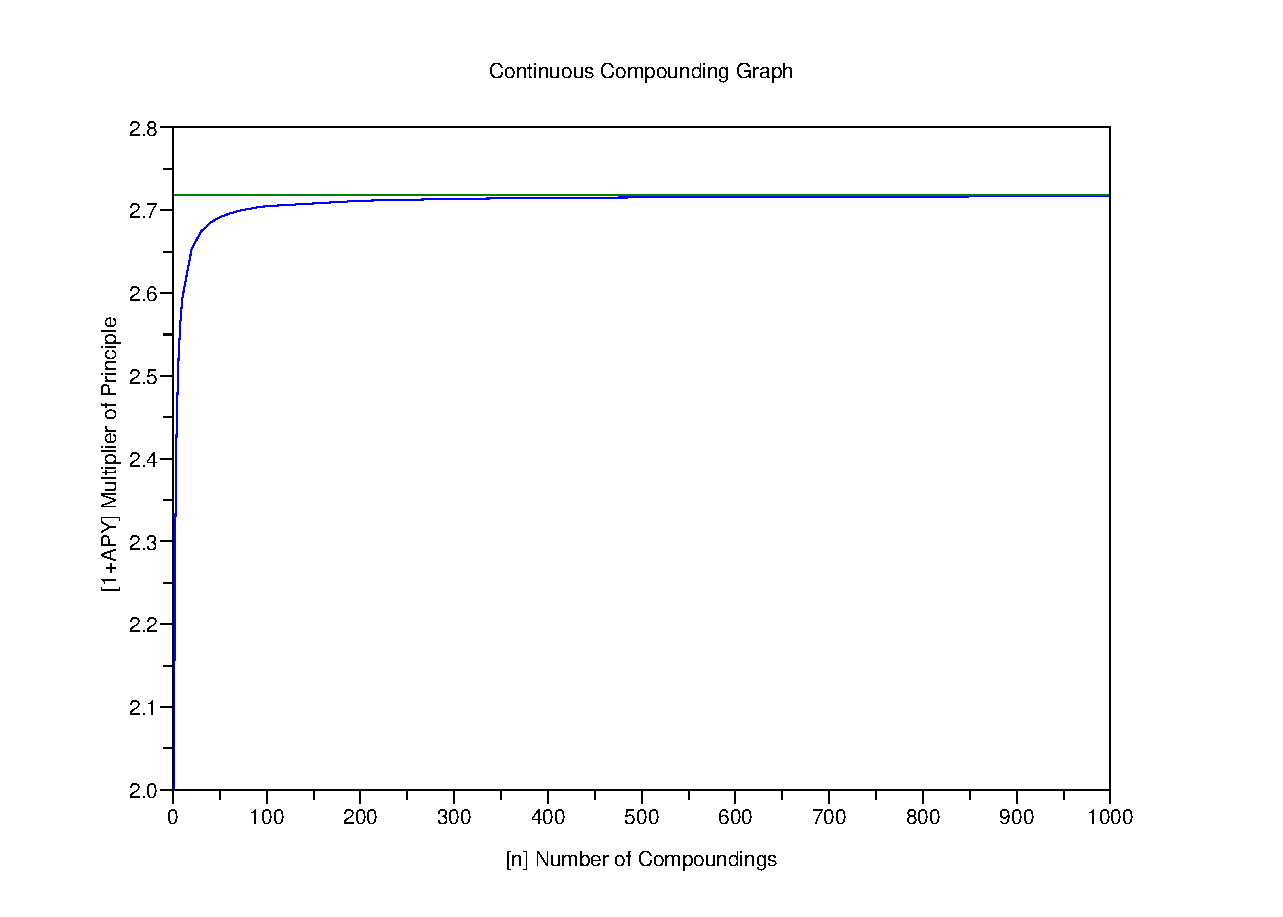
\includegraphics[width=4.4in]{contcomp.eps}}
\end{tabular}
\vspace{.1in}
\end{center}
\end{figure*}


The final term is a special number in mathematics called $e$.  There are many similarities between the constants $e$ and $\pi$. Here are a few.
\begin{enumerate}
\item Both arise naturally in calculations.  Circles, curves, and angles give rise to $\pi$, while compounding and calculus operations on exponents give rise to $e$.
\item Both numbers are not rational, which means they cannot be expressed as the ratio of integers.
\item Both numbers are not algebraic and thus they are transcendental.  An algebraic number is one which can be expressed as the root of a polynomial with integer coefficients.
\item Both have no repeating patterns in their decimal expansion.  This is a result of being irrational.
\end{enumerate}

\subsection{Fun with Numbers}

I thought I would take this time to give you a little taste of Number Theory.  This is the type of thing which mathematicians find fun.  Lets look a few of them.

First, consider a repeating decimal like 0.345345345�  We would like to know how to express this as a fraction.  We know 345/1000 gives us 0.345, which is a little smaller than we want, so we make the denominator a little smaller.  We try 345/999 and we find that indeed we get the desired result.  Try the following

\begin{tabular}{cccc}
7/9 & 75/99 & 752/999 & 7528/9999 \\
5/9 & 50/99 & 504/999 & 5046/9999 \\
1/9 & 12/99 & 123/999 & 1234/9999
\end{tabular}

Why does this work?  Consider the following.

Let some number sequence of $n+1$ digits be given by $d_0d_1\cdots d_n$.  To make it easy to follow note that $n+1$ digits of all 9's is specified by $9_09_1\cdots 9_n$.  Finally we will look at the ratio,
\begin{eqnarray*}
x&=& \frac{d_0d_1\cdots d_n}{9_09_1\cdots 9_n} \\
 &=& \frac{d_0d_1\cdots d_n}{10^{n+1}-1}\\
% &=& \frac{d_0d_1\cdots d_n}{10^{n+1}-1}\frac{10^{n+1}}{10^{n+1}}\\
% &=& \frac{d_0d_1\cdots d_n}{10^{n+1}}\frac{10^{n+1}-1+1}{10^{n+1}-1}\\
% &=& \frac{d_0d_1\cdots d_n}{10^{n+1}}\left(1+\frac{1}{10^{n+1}-1}\right)\\
% &=& \frac{d_0d_1\cdots d_n}{10^{n+1}}+\frac{d_0d_1\cdots d_n}{10^{n+1}}\frac{1}{10^{n+1}-1}\\
% &=& 0.d_0d_1\cdots d_n+\frac{d_0d_1\cdots d_n}{10^{n+1}-1}\frac{1}{10^{n+1}}\\
x(10^{n+1}-1) &=& d_0d_1\cdots d_n\\
x10^{n+1} &=& d_0d_1\cdots d_n+x\\
x &=& \frac{d_0d_1\cdots d_n}{10^{n+1}}+x\frac{1}{10^{n+1}}\\
  &=& 0.d_0d_1\cdots d_n+x\frac{1}{10^{n+1}}
\end{eqnarray*}
Think about what this equation means.  The ratio, $x$, is equal to a fixed length ($n+1$ digits) decimal number and a shifted (by $n+1$) copy of itself.  Since the shift is equal to the size of the fixed number, they don't overlap.  We can then see that this can be handled recursively, see Table~\ref{tab-digit-recursion}.
\begin{table*}[t]
\begin{center}
\caption{Digit recursion.}\label{tab-digit-recursion}
\noindent
\begin{tabular}{lp{3in}}
x & explanation \\\hline
$0.d_0d_1\cdots d_n$ & The first $n+1$ digits must be from the fixed number since the shift is large enough so there is no overlap. \\
$0.d_0d_1\cdots d_n\;d_0d_1\cdots d_n$ & Since we know the first $n+1$ digits, we know from the shift term that the first $n+1$ digits are copied and shifted to the second $n+1$ digits. \\
$0.d_0d_1\cdots d_n\;d_0d_1\cdots d_n\;d_0d_1\cdots d_n$ & Since we know the second $n+1$ digits, we know from the shift term that the second $n+1$ digits are copied and shifted to the third $n+1$ digits. \\
$\qquad\vdots$ & The process repeats, generating the pattern.
\end{tabular}
\end{center}
\end{table*}

\noindent
Note the term in square brackets is repeat of the term on the on line two so we have for 345/999, that it is 0.345(1.001001\ldots) or 0.345345345\ldots  We have seen that this works in general.  Try 9/9.  We should see 0.99999� from what we have shown, but we see 1!  Why?  Well, 1=0.99999\ldots! Here is an easy way to see this.
\begin{eqnarray*}
y &=& 0.999\cdots \\
10y &=& 9.999\cdots \\
10y-y &=& 9.999\cdots - 0.999\cdots \\
9y &=& 9 \\
y &=& 1
\end{eqnarray*}
An amazing result!  Anyway, I hope this little diversion sparks an interest in number theory.

\subsection{Amortization and Savings}
Up till now we have looked at a single starting value and what it will be worth (or cost).  Now we will consider amortization and regular payments.  Say we are going to make regular payments of $A$ for $m$ periods per year and $n$ years.  Further, say you will get $r=\frac{i}{m}$ as an interest rate.  We can treat this as a bunch of compounded equations that are added together.
\begin{eqnarray}
F &=& A(1+r)^{nm-1}+ A(1+r)^{nm-2}+ \nonumber\\
  &&\qquad \ldots+A(1+r)+A \nonumber\\
  &=& \sum_{k=0}^{nm-1}A(1+r)^k \nonumber\\
  &=& A\sum_{k=0}^{nm-1}(1+r)^k
\end{eqnarray}
Note that this is nice looking series, so we might suspect there is an easier way of summing.  Consider the series
\begin{eqnarray}
s_{m}(x)&=&\sum_{k=0}^{m-1}x^k,
\end{eqnarray}
then multiply by $\frac{(x-1)}{(x-1)}$ to obtain
\begin{eqnarray}
s_{m}(x) &=& \frac{xs_{m}(x)-s_{m}(x)}{x-1} \nonumber\\
         &=& \frac{x\left(x^{m-1}+s_{m-1}(x)\right)}{x-1}\nonumber\\
         &&\;-\frac{\left(xs_{m-1}(x)+1\right)}{x-1} \nonumber\\
         &=& \frac{x^m+xs_{m-1}(x)}{x-1}\nonumber\\
         &&\;-\frac{xs_{m-1}(x)-1}{x-1} \nonumber\\
         &=& \frac{x^m-1}{x-1}.
\end{eqnarray}
We note that for us $x=1+r$ so we have
\begin{eqnarray}
F &=& A\sum_{k=0}^{nm-1}(1+r)^k \nonumber\\
  &=& A\frac{(1+r)^{nm}-1}{(1+r)-1} \nonumber\\
  &=& A\frac{(1+r)^{nm}-1}{r}\nonumber\\
\frac{F}{A} &=& \frac{(1+r)^{nm}-1}{r} \\
&=& \left(\frac{F}{A},\;r,\;nm\right).
\end{eqnarray}
This is called the amortization or savings formula.

When paying off a mortgage or loan, the future value of the amortization (your payment) and the future value of the initial amount of the loan are set equal.  Assuming multiple compoundings we have
\begin{eqnarray}
P(1+r)^{nm} &=& A\frac{(1+r)^{nm}-1}{r} \nonumber\\
          A &=& \frac{P(1+r)^{nm}r}{(1+r)^{nm}-1} \nonumber\\
\frac{A}{P} &=& \frac{r(1+r)^{nm}}{(1+r)^{nm}-1} \nonumber\\
            &=& \left(\frac{A}{P},\;r,\;nm\right). \label{eq-cap-recovery}
\end{eqnarray}
The final equation (eq.~\ref{eq-cap-recovery}) is called the \textbf{Capital Recovery Factor}, and it is tabulated for various values of interest and compounding periods.  Notice that this is the formula used for loans (loan value is $P$, monthly payment is $A$, and the number of monthly payments is $nm$).  The reciprocal,
\begin{eqnarray}
\frac{P}{A} &=& \frac{(1+r)^{nm}-1}{r(1+r)^{nm}} \\
            &=& \left(\frac{P}{A},\;r,\;nm\right),
\end{eqnarray}
is also an important equation, and is called the \textbf{Present Worth Factor, Uniform Series}.

\subsection{Arithmetic Gradients}

\subsubsection{Compound amount, arithmetic gradient}
\begin{eqnarray}
\frac{F}{G} &=& \left(\frac{(1+r)^k-(1+rk)}{r^2}\right) \\
            &=& \left(\frac{F}{G},\;r,\;k\right)
\end{eqnarray}

\subsubsection{Present worth factor, arithmetic gradient}
\begin{eqnarray}
\frac{P}{G} &=& \left(\frac{(1+r)^k-(1+rk)}{r^2(1+r)^k}\right) \\
            &=& \left(\frac{P}{G},\;r,\;k\right)
\end{eqnarray}

\subsubsection{Annuity factor, arithmetic gradient}
\begin{eqnarray}
\frac{A}{G} &=& \left(\frac{(1+r)^k-(1+rk)}{r(1+r)^k-r}\right) \\
            &=& \left(\frac{A}{G},\;r,\;k\right)
\end{eqnarray}


\subsection{Conversion}

Let's summarize our conversion factors.  Note that often we have combinations of terms to describe some situation, but with our conversion table we can handle this.

\begin{tabular}{c|cccc}
   & \multicolumn{4}{c}{From} \\
To & P                                   & F                            & A                                   & G \\\hline
P  & 1                                   & $(1+r)^{-k}$                 & $\frac{(1+r)^k-1}{r(1+r)^k}$        & $\frac{(1+r)^k-(1+rk)}{r^2(1+r)^k}$ \\
F  & $(1+r)^k$                           & 1                            & $\frac{(1+r)^k-1}{r}$               & $\frac{(1+r)^k-(1+rk)}{r^2}$ \\
A  & $\frac{r(1+r)^k}{(1+r)^k-1}$        & $\frac{r}{(1+r)^k-1}$        & 1                                   & $\frac{(1+r)^k-(1+rk)}{r(1+r)^k-r}$ \\
G  & $\frac{r^2(1+r)^k}{(1+r)^k-(1+rk)}$ & $\frac{r^2}{(1+r)^k-(1+rk)}$ & $\frac{r(1+r)^k-r}{(1+r)^k-(1+rk)}$ & 1           \\
\end{tabular}

As odd as it might sound, we often prefer to use just the labels, because we can tabulate or do function calls to get the solution, which tends to be less error prone than doing arithmetic.  See Appendix~\ref{ch-econ-tables} for sample compound interest table factors.

\begin{tabular}{c|cccc}
   & \multicolumn{4}{c}{From} \\
To & P           & F           & A           & G \\\hline
P  & 1           & $(P/F,r,k)$ & $(P/A,r,k)$ & $(P/G,r,k)$ \\
F  & $(F/P,r,k)$ & 1           & $(F/A,r,k)$ & $(F/G,r,k)$ \\
A  & $(A/P,r,k)$ & $(A/F,r,k)$ & 1           & $(A/G,r,k)$ \\
G  & $(G/P,r,k)$ & $(G/F,r,k)$ & $(G/A,r,k)$ & 1           \\
\end{tabular}


\section{Returns and Comparison Methods}
\subsection{Equivalent Uniform Annual Cost(EUAC)}
\begin{eqnarray}
EUAC &=& \left(\frac{A}{P},\;r,\;k\right)P \nonumber\\
     &&\;-\left(\frac{A}{F},\;r,\;k\right)S
\end{eqnarray}
where $P$ is the cost of the item, and $S$ is the salvage value (what can you sell it for when you are done).


\subsection{Equivalent Uniform Annual Benefit(EUAB)}
\begin{eqnarray}
EUAB &=& A-\left(\frac{A}{P},\;r,\;k\right)P
\end{eqnarray}
where $P$ is the cost of the investment, and $A$ is the periodic return.

\subsection{Net Present Worth(NPW)}
Net present worth (NPW) is defined by
\begin{eqnarray}
NPW &=& \left(\frac{P}{A},\;r,\;k\right)A-P
\end{eqnarray}
where $P$ is the cost of the investment, and $A$ is the periodic return.


\subsection{Rate of Return(ROR)}
The rate of return is the interest rate, which makes the net present worth equal zero.  The rate of return is thus:
\begin{eqnarray}
ROR &=& r \nonumber\\
    &&\; s.t.\;NPW=0,
\end{eqnarray}
where $s.t.$ means ``such that''\footnote{Such that means that there is a constraint that must be fulfilled.  It is frequently used in constrained minimization, but can be used - as it is here - to specify a one parameter system from which any solution will do.}.  ROR is usually evaluated with respect to a minimum attractive rate of return (MARR), which is selected to reflect current options and relative risk of the investment.  MARR can be selected to be a safe investment's ROR (such as a savings account or secure bonds).



\section{Depreciation}
We have seen how things grow.  We also need to see how things lose value.  Major assets (homes, cars, computers, etc.) do not retain their value.  They get used and thus worth less to others, some more than others.  For instance, cars tend to lose 25\% of their value a year until they are in the \$1000 range where they tend to hover (unless they are a classic).  Houses on the other hand tend not to lose a lot of value and actually start gaining value after about 5-10 years of age.   Depreciation works just like interest, except the rate is negative.

Consider a new car that costs \$20,000 and loses 25\% of its value each year.  How much is it worth in 1, 2, 5, 10 years?

\begin{tabular}{rcl}
Years & Formula              & Value \\ \hline
0     & $20000(1-0.25)^0$    & \$20,000 \\
1     & $20000(1-0.25)^1$    & \$15,000 \\
2     & $20000(1-0.25)^2$    & \$11,250 \\
5     & $20000(1-0.25)^5$    & \$4,746 \\
10    & $20000(1-0.25)^{10}$ & \$1,126 \\
\end{tabular}

People often find it difficult to calculate this, so other methods are often used.  Some of the most common are below.

\subsection{Straight Line Depreciation}
\begin{eqnarray}
D_k=\frac{C-S}{n}
\end{eqnarray}
where $D_k$ is the depreciation in year $k$, $C$ is the cost of the item, $S$ is the salvage value (what you get for selling it at the end, and $n$ is the number of years till you salvage it.

\subsection{Accelerated Cost Recovery System (ACRS)}
\begin{eqnarray}
D_k=W_j(C-S)
\end{eqnarray}
where $D_k$ is the depreciation in year $k$, $C$ is the cost of the item, $S$ is the salvage value (what you get for selling it at the end, and $W_j$ is from Table~\ref{tab-acrs-weights}.
\begin{table}[h]
\caption{ACRS Weights}\label{tab-acrs-weights}
\begin{tabular}{ccccc}
&\multicolumn{4}{c}{Recovery Period}\\
Year & 3    & 5    & 7    & 10   \\ \hline
1    & .333 & .200 & .143 & .100 \\
2    & .445 & .320 & .245 & .180 \\
3    & .148 & .192 & .175 & .144 \\
4    & .074 & .115 & .125 & .115 \\
5    &      & .115 & .089 & .092 \\
6    &      & .058 & .089 & .074 \\
7    &      &      & .089 & .066 \\
8    &      &      & .045 & .066 \\
9    &      &      &      & .065 \\
10   &      &      &      & .065 \\
11   &      &      &      & .033 \\
\end{tabular}
\end{table}






\section{Resources}
\subsection{Non-Renewable Resources}
If you have a sum of money, a quantity of oil, etc., that you cannot replace then it is a non-renewable resource.  There are two ways you can use it (in practical situation, theoretically you can use it in infinitely many ways).  Our primary interest is when the resource will be used up.

The first is static consumption.  In it you use the same amount, A, every period.  The resource will last
\begin{eqnarray}
t_s &=& \frac{P}{A}
\end{eqnarray}
The second type is exponential consumption.  In it you start by using A the first period, and then you use A(1+r) the next period, and so on.  The equation ends up looking like the savings formula (though we are withdrawing not depositing).  In any case the formula is
\begin{eqnarray*}
P &=& A + A(1+r) + \dots + A(1+r)^{t_e-1}\\
  &=& A\frac{(1+r)^{t_e}-1}{r}
\end{eqnarray*}
We can then solve for $t_e$, the time when it is all gone.
\begin{eqnarray}
\frac{P}{A}r+1  &=& (1+r)^{t_e}\\
\ln\left(\frac{P}{A}r+1\right)  &=& t_e\ln(1+r)\\
t_e &=& \frac{\ln\left(\frac{P}{A}r+1\right)}{\ln(1+r)}
\end{eqnarray}

\subsection{Renewable Resources}
If you have a sum of money, a group of animals, an amount of plants, etc., that can grow, you have a renewable resource.  In this case it makes sense to live off the surplus amount above that which is needed to maintain the quantity at current levels.  For money you live off the interest.

If we ignore inflation the amount we get in one year is given by
\begin{eqnarray}
F &=& P(1+r)\\
  &=& P+rP.
\end{eqnarray}
We want to keep an amount P left over (for the following year) so the net gain (what we can live off) is
\begin{eqnarray}
A &=& F-P \\
  &=& P+rP- P\\
  &=& rP.
\end{eqnarray}
We might want to consider inflation into this equation, so the money we have to spend each year remains of equal value.  In this case the amount we need to keep from spending is $P(1+i)$, which gives us an amount to live off of
\begin{eqnarray}
A &=& F-P(1+i) \\
  &=& P+rP- P-iP\\
  &=& (r-i)P.
\end{eqnarray}
Since interest rates are determined by inflation (usually r=i+1\% to 3\%).  For instance it is reasonable to assume that if you live off $\frac{1}{50}$ of an amount you can do so forever.



\section{Estimating Costs}

\subsection{Engineering Cost Estimate Method}
A bottom-up method that consists of estimating the costs for each sub area (labor, materials, overhead, etc.).  Very detailed and often quite accurate.  Costs are assigned to each definable task or activity in the work breakdown structure (WBS).

\subsection{Roundtable Cost Estimate Method}
Experts representing every discipline/area of the production meet to discuss cost based on experience.  Typically this includes engineering (hardware, software, mechanical), manufacturing (production, assembly), flight test/quality assurance, logistics \& purchasing, accounting, contracts, and human resources.

\subsection{Actual Costs Extrapolation Method}
Calculate the cost from prototype costs.  This is very accurate but can't always be done and is not available early in the process.

\subsection{Analogy Cost Estimating Method}
Draws an analogy to an existing product, and uses the costing of the existing product.  Differences can be specified, and cost modifiers used.  This is the simplest method, and its accuracy requires that good historical data be available, a proper analogy drawn, and differences properly noted.  It is not only simple, it can also be fast, and usually provides a good rough order of magnitude.

\subsection{Parametric/Statistical Estimation Method}
Use a database of similar systems to generate estimates of the cost.  This is essentially a multiple item analogy cost estimate.  Often used early in the design process.  In this method we exploit correlation of variables.  When considering why variables have a high correlation/relation in the data (indicating a potential dependence), there are three possible reasons:
\begin{enumerate}
\item No relation - it is chance.
\item Related but not causal - neither one caused the other, but some relation exists between the variables.
    \begin{enumerate}
    \item All dependent on missing variable.  For example let $x$ and $y$ be two variables which exhibit a relation.  It is possible that both are dependent and there is a missing independent variable, say $t$, such that $x=f(t)$ and $y=g(t)$.  One such case is that of the amount of sunlight in two different places on the earth.  It being daylight in LA does not cause it to be night in Mumbai, though it will be the case due to a missing variable.  The shape and rotation of the earth causes the day/night phenomena noted.
    \item They might be co-dependent, as you often see in symbiotic relations among plants and animals.  Thus $x=f(y)$ and $y=g(x)$ and we cannot tell which is independent (and there often isn't one).
    \item The might be two independent factors, where a joint distribution is known thus constraining them, but not being dependent in a causal way.  For example $z=f(x,y)$, if we know the function and values of z, it will constrain the $x$ and $y$ used to pick it.
    \end{enumerate}
\item Causal - one variable caused the other to take on the value, such as an unbalanced force causing an acceleration.
\end{enumerate}
Often we can get away with a linear fit, which has the virtue of being easy to calculate. To see how good this is we can use several goodness of fit measures.
\begin{description}
\item[Residual]  The sum of all the errors of fit, measured only in the dependent variable's direction.  Also called standard error or standard error of estimate (not to be confused with statistical error).
\item[Coefficient of Variation of Residuals] Useful in comparing distributions with widely varying stats.  See Appendix~\ref{ch-stats}.
\item[Correlation Coefficient] The covariance of the two variables divided by the variables standard deviations, see Appendix~\ref{ch-stats}.
\item[Determination Coefficient] The square of the correlation coefficient.
\end{description}


